
\newpage
 

\subsection*{Financial Health}

\begin{figure}[h]
    \centering
    \begin{subfigure}{0.48\textwidth}
        \centering
        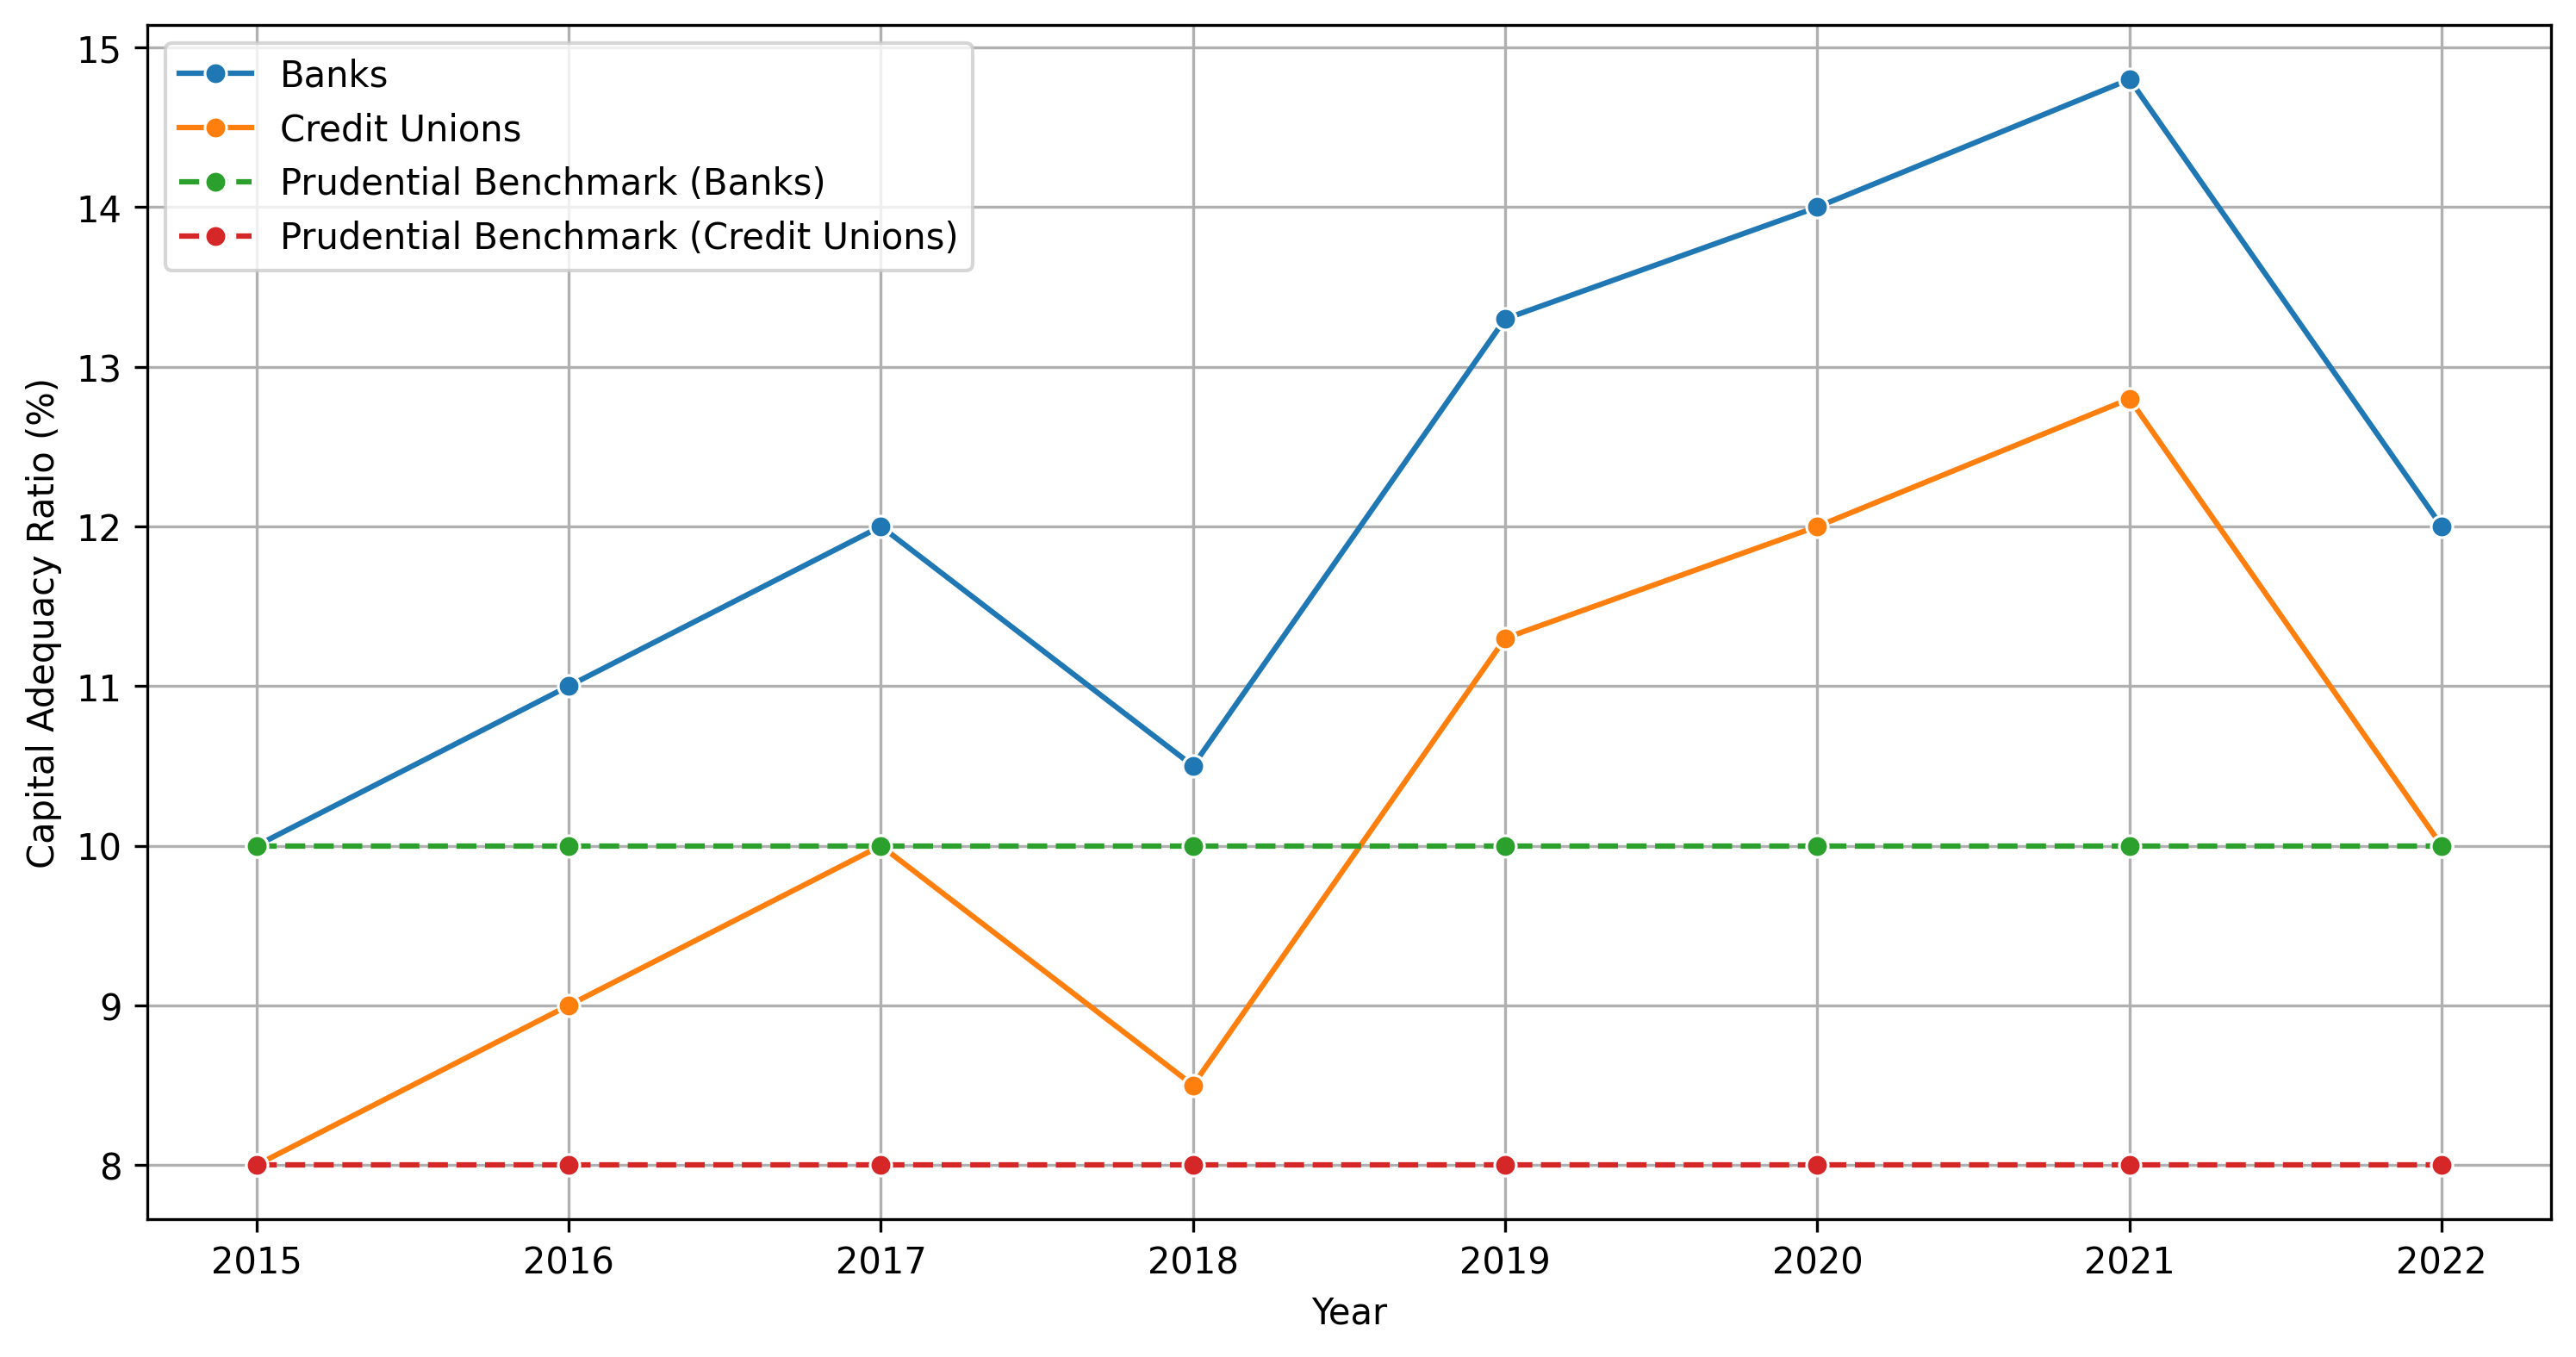
\includegraphics[width=\textwidth]{Benchmarks.png}
        \caption{\small Credit Extended by Banks and Credit Unions}
        \label{fig:benchmarks}
    \end{subfigure}
    \hfill
    \begin{subfigure}{0.48\textwidth}
        \centering
        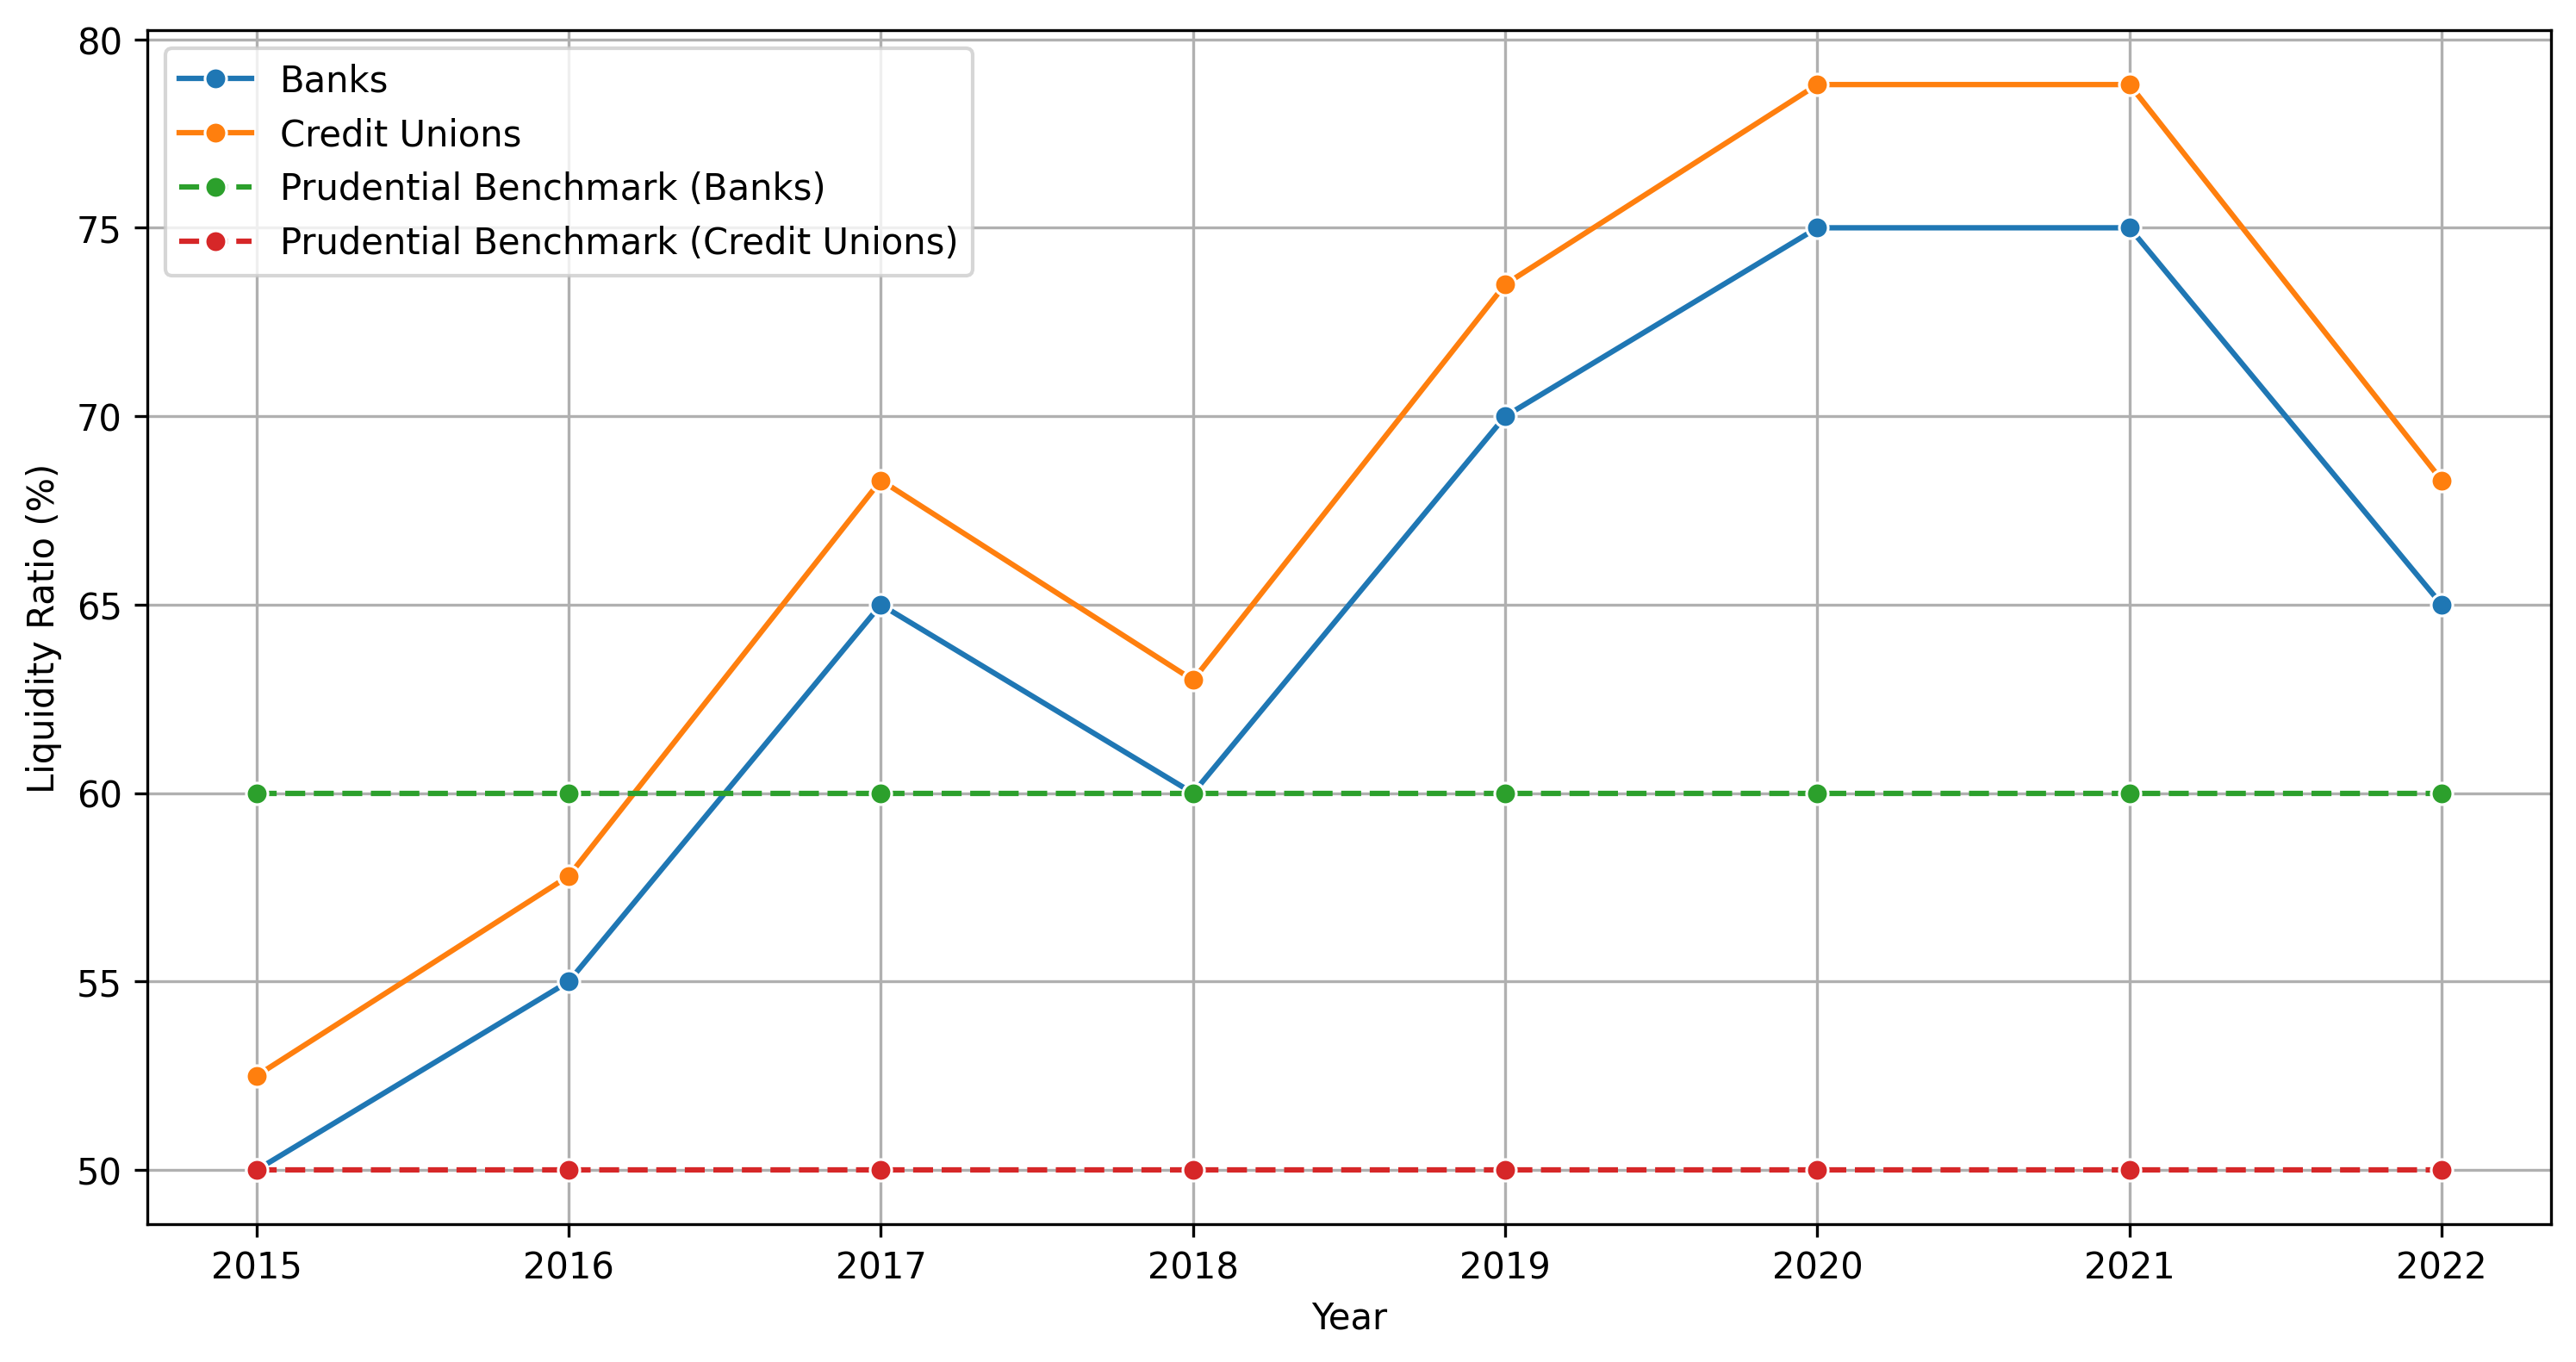
\includegraphics[width=\textwidth]{liquidity_ratio.png}
        \caption{\small Liquidity Ratios for Banks and Credit Unions}
        \label{fig:liquidity_ratios}
    \end{subfigure}
    \caption{Banking Sector Credit and Liquidity Ratios}  % Main figure caption
    \label{fig:credit_liquidity}
\end{figure}



Nominally, Macaronia's \textcolor{teal}{liquidity} and \textcolor{teal}{capital adequacy ratios} are both above the set \textcolor{teal}{prudential benchmarks}.  
Over the years, \textcolor{teal}{banks} and \textcolor{teal}{credit unions} have attained \textcolor{teal}{liquidity ratios} of \textbf{\textcolor{teal}{75\%}} (a \textbf{\textcolor{teal}{25\% increase}})  
and \textbf{\textcolor{teal}{78.8\%}} (a \textbf{\textcolor{teal}{26.3\% increase}}), respectively.  
Similarly, \textcolor{teal}{capital adequacy ratios} have reached \textbf{\textcolor{teal}{14.8\%}} (a \textbf{\textcolor{teal}{4.8\% increase}}) for \textcolor{teal}{banks}  
and \textbf{\textcolor{teal}{12.8\%}} (a \textbf{\textcolor{teal}{4.8\% increase}}) for \textcolor{teal}{credit unions}.  
On paper, these ratios appear strong, suggesting that \textcolor{teal}{financial institutions} are \textcolor{teal}{solvent}  
and have sufficient \textcolor{teal}{liquidity} to meet \textcolor{teal}{short-term obligations}.


However, much like inflation erodes the real value of money, the effectiveness of these ratios is being 
undermined by the rapid expansion of credit. While the ratios are rising, the scale of credit being extended 
to Macaronia's households has grown at a significant rate as well. For instance:

\begin{itemize}
    \item \textbf{\textcolor{teal}{Credit extended by banks}} grew from \textbf{\textcolor{teal}{1.5\% in 2015}} to \textbf{\textcolor{teal}{8.8\% in 2021}}.
    \item \textbf{\textcolor{teal}{Credit extended by credit unions}} grew from \textbf{\textcolor{teal}{2.3\% in 2015}} to \textbf{\textcolor{teal}{13.3\% in 2021}}.
\end{itemize}

This rapid growth in credit is evidenced by the strong correlations between 
\textbf{credit extended by banks (0.92)} and \textbf{credit unions (0.86)} with their respective 
solvency ratios, as well as between \textbf{credit extended by banks (0.91)} and \textbf{credit unions (0.81)} 
with their respective liquidity ratios.

\begin{figure}[h]     
     \centering
     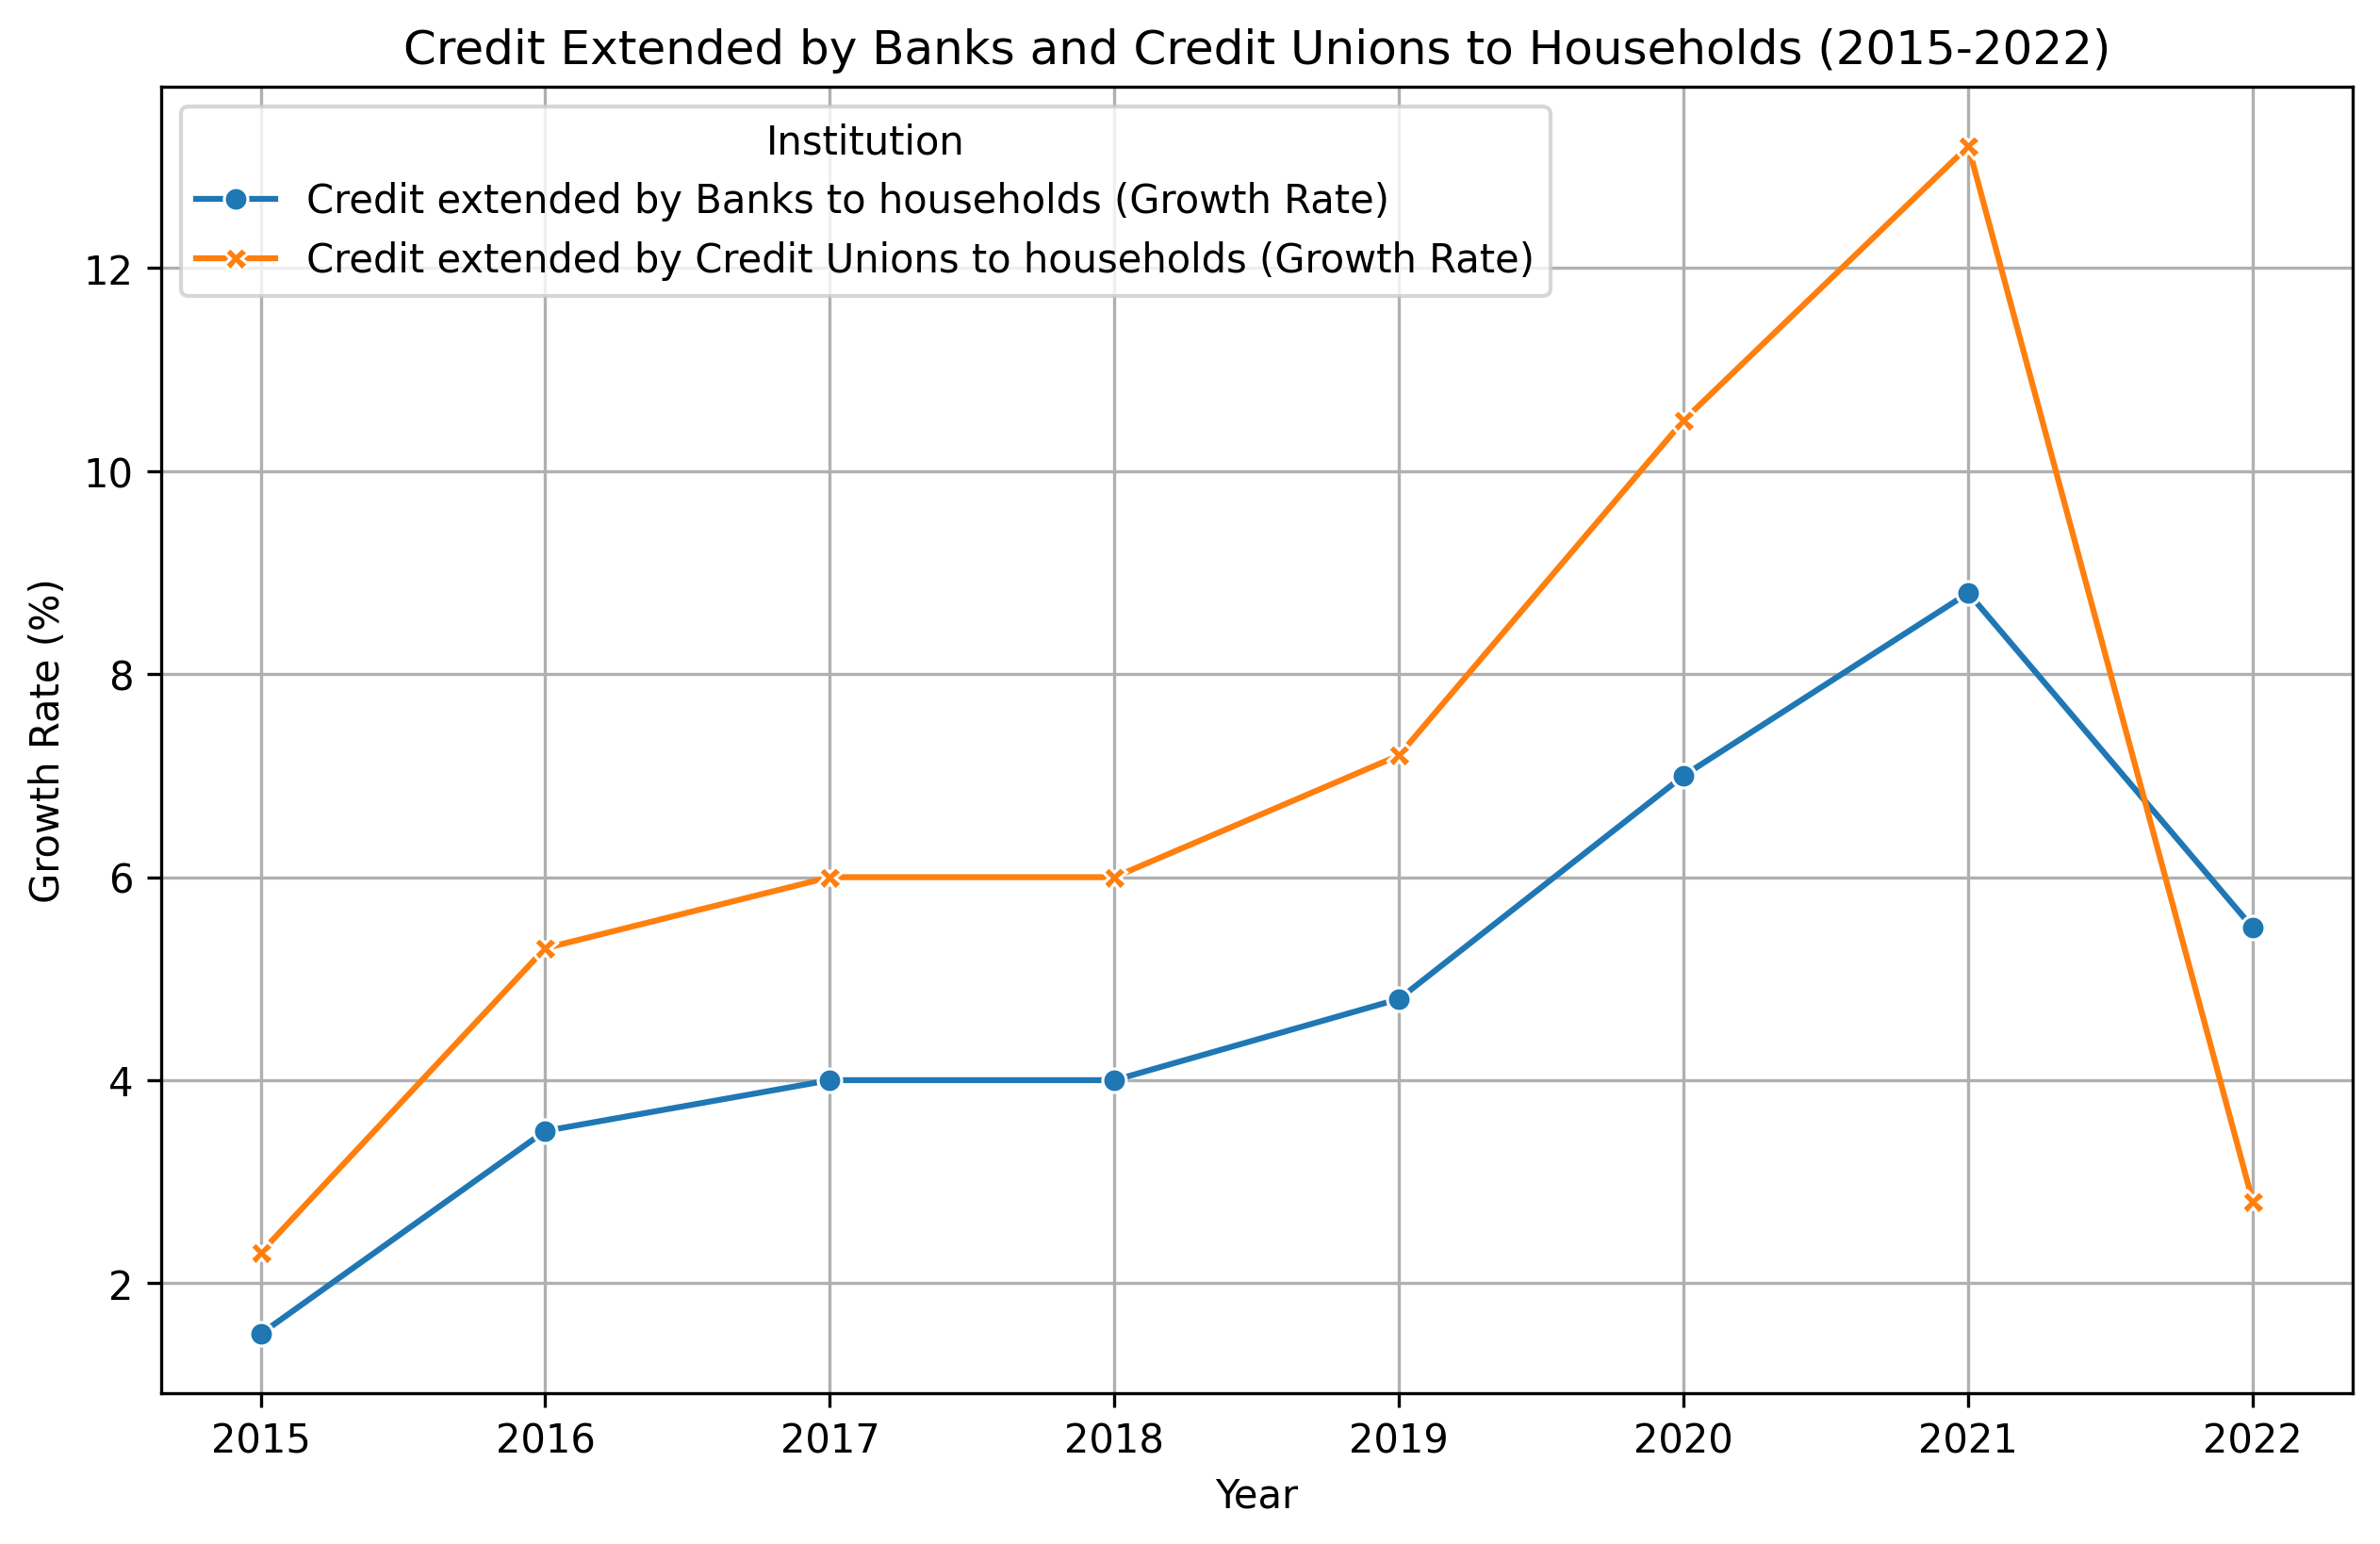
\includegraphics[width=0.53\textwidth]{graph_1.png}
     \caption{Credit Extended By Banks and Credit Unions to Households (2015 - 2022)}
     \label{fig:graph_1}
\end{figure}

To make matters worse, both banks and credit unions in Macaronia are heavily exposed to \textbf{\textcolor{teal}{Real Estate Investment Trusts (REITs)}}, 
with banks having \textbf{\textcolor{teal}{15\%}} of their assets tied to REITs, and credit unions having \textbf{\textcolor{teal}{25\%}}. 
REITs are highly volatile, with their values subject to significant fluctuations based on market conditions, 
interest rates, and economic cycles. In times of economic uncertainty, these assets put financial institutions
in a precarious position, as they would struggle to meet their short-term obligations in the event of a bank run
or an external shock.  \textcolor{orange}{\cite{FSB2023GlobalMonitoring}}


\begin{figure}[h]
    \centering
    \begin{subfigure}{0.48\textwidth}
        \centering
        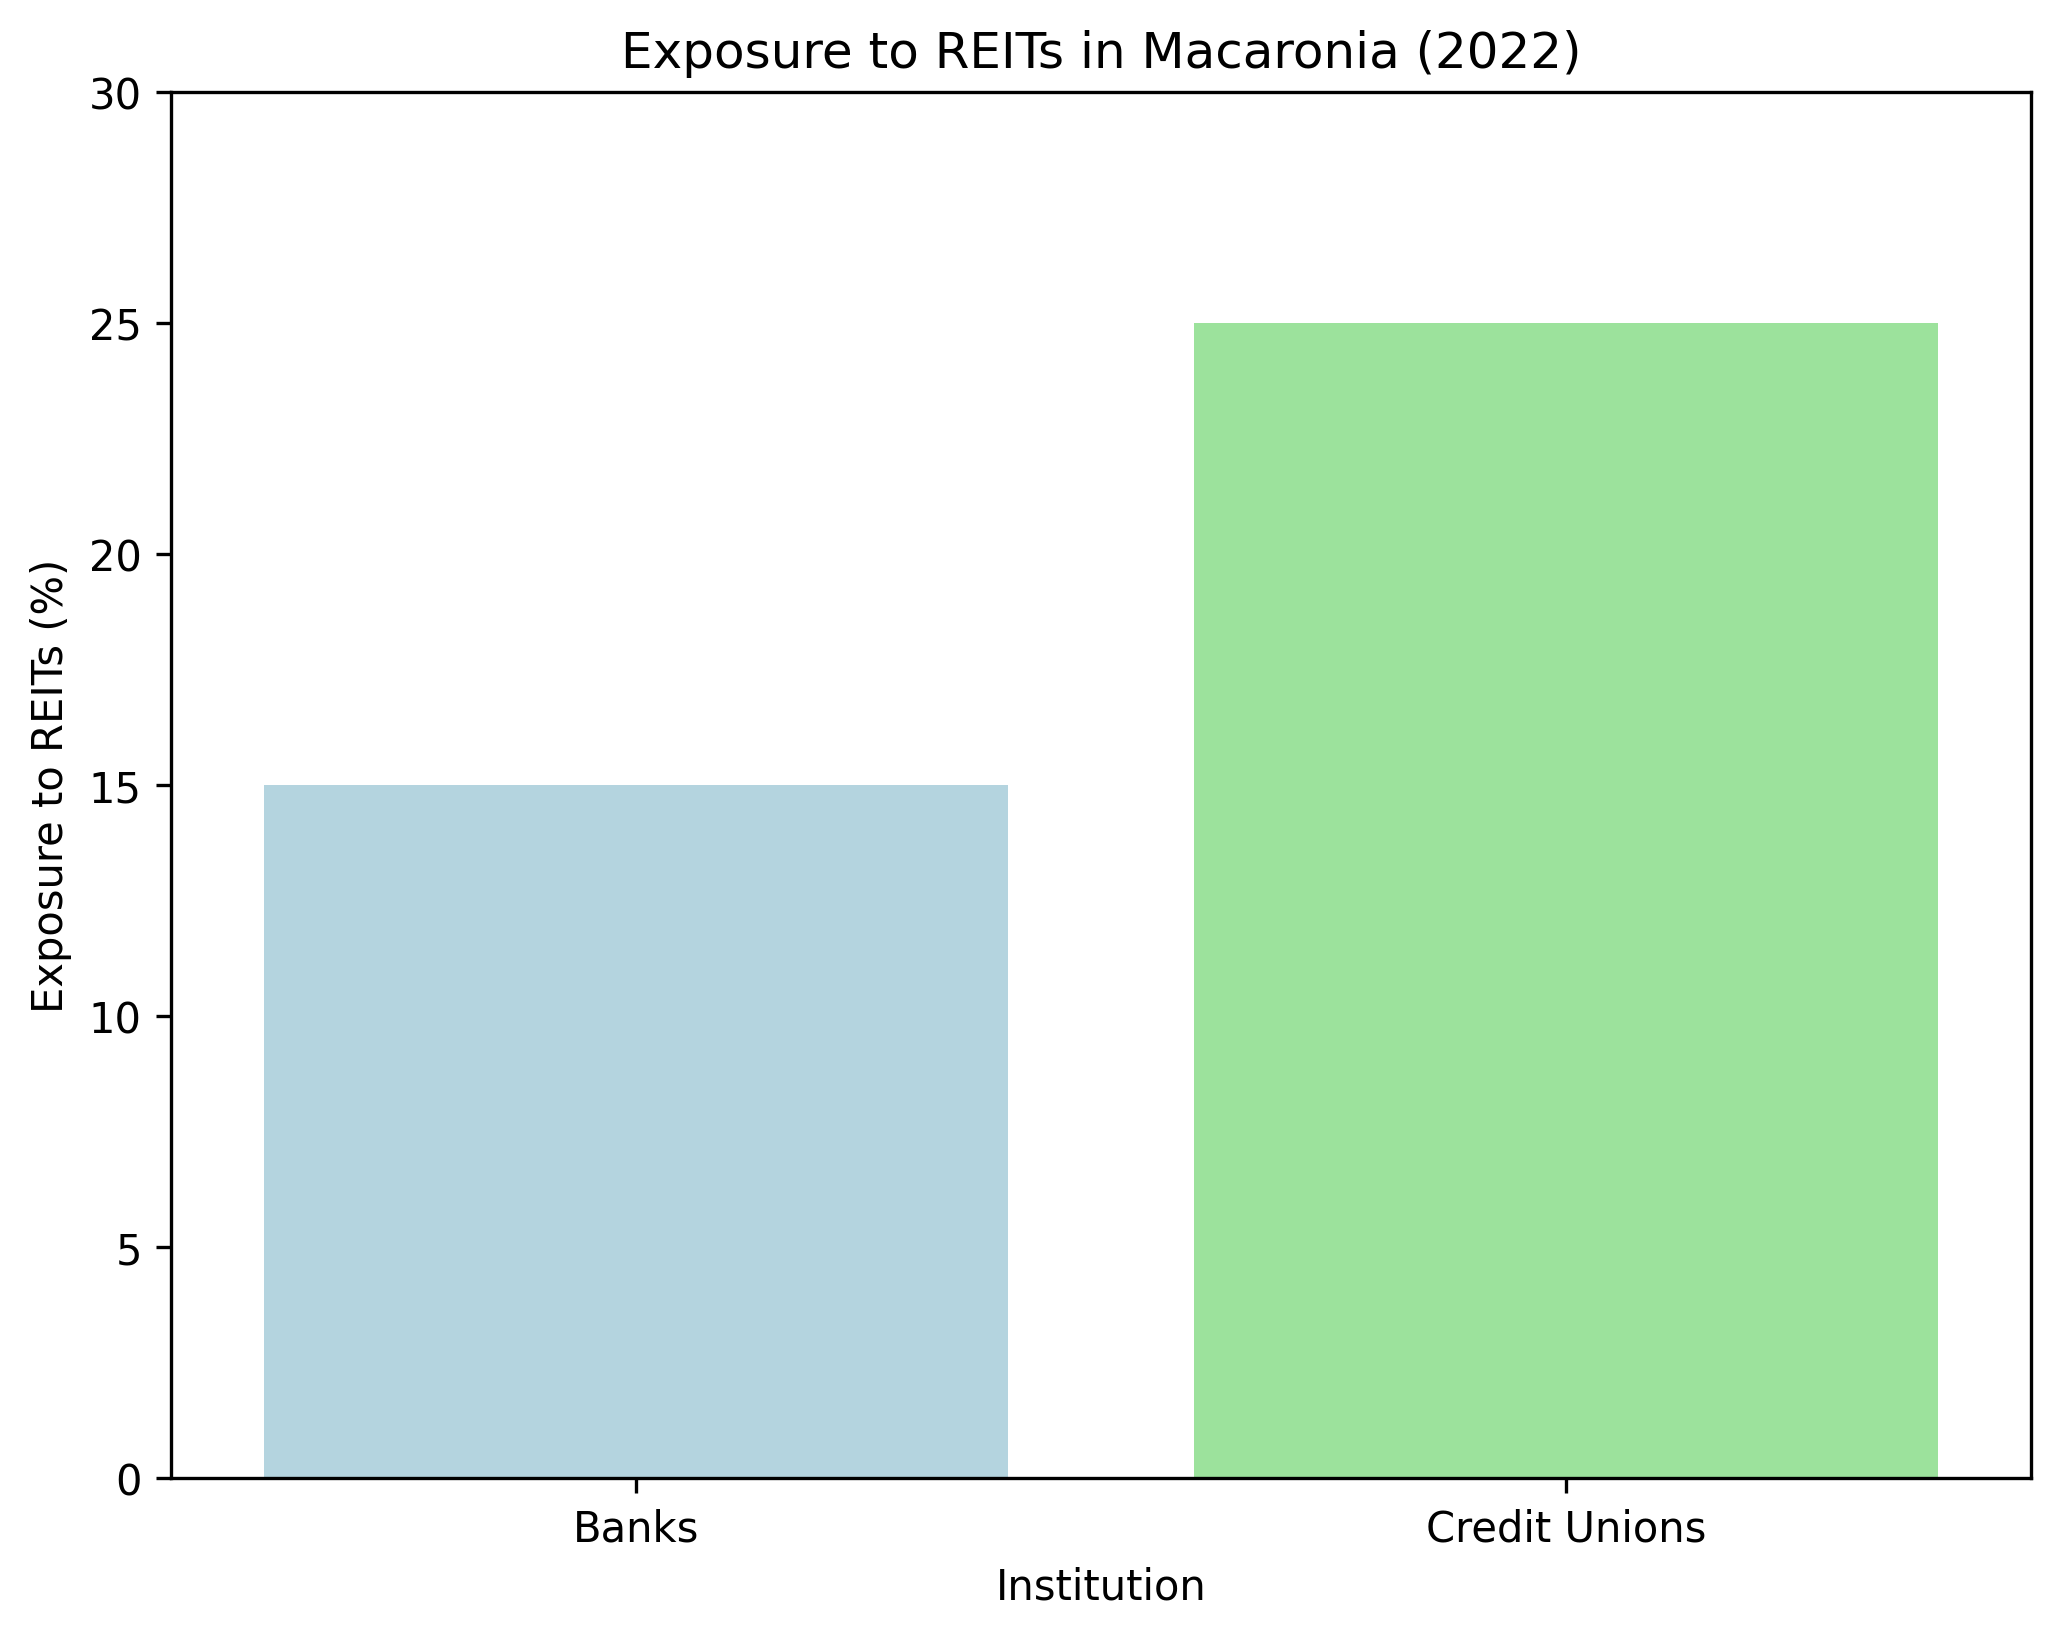
\includegraphics[width=\textwidth]{REIT.png}
        \caption{\small REIT Exposure}
        \label{fig:reit_exposure}
    \end{subfigure}
    \hfill
    \begin{subfigure}{0.48\textwidth}
        \centering
        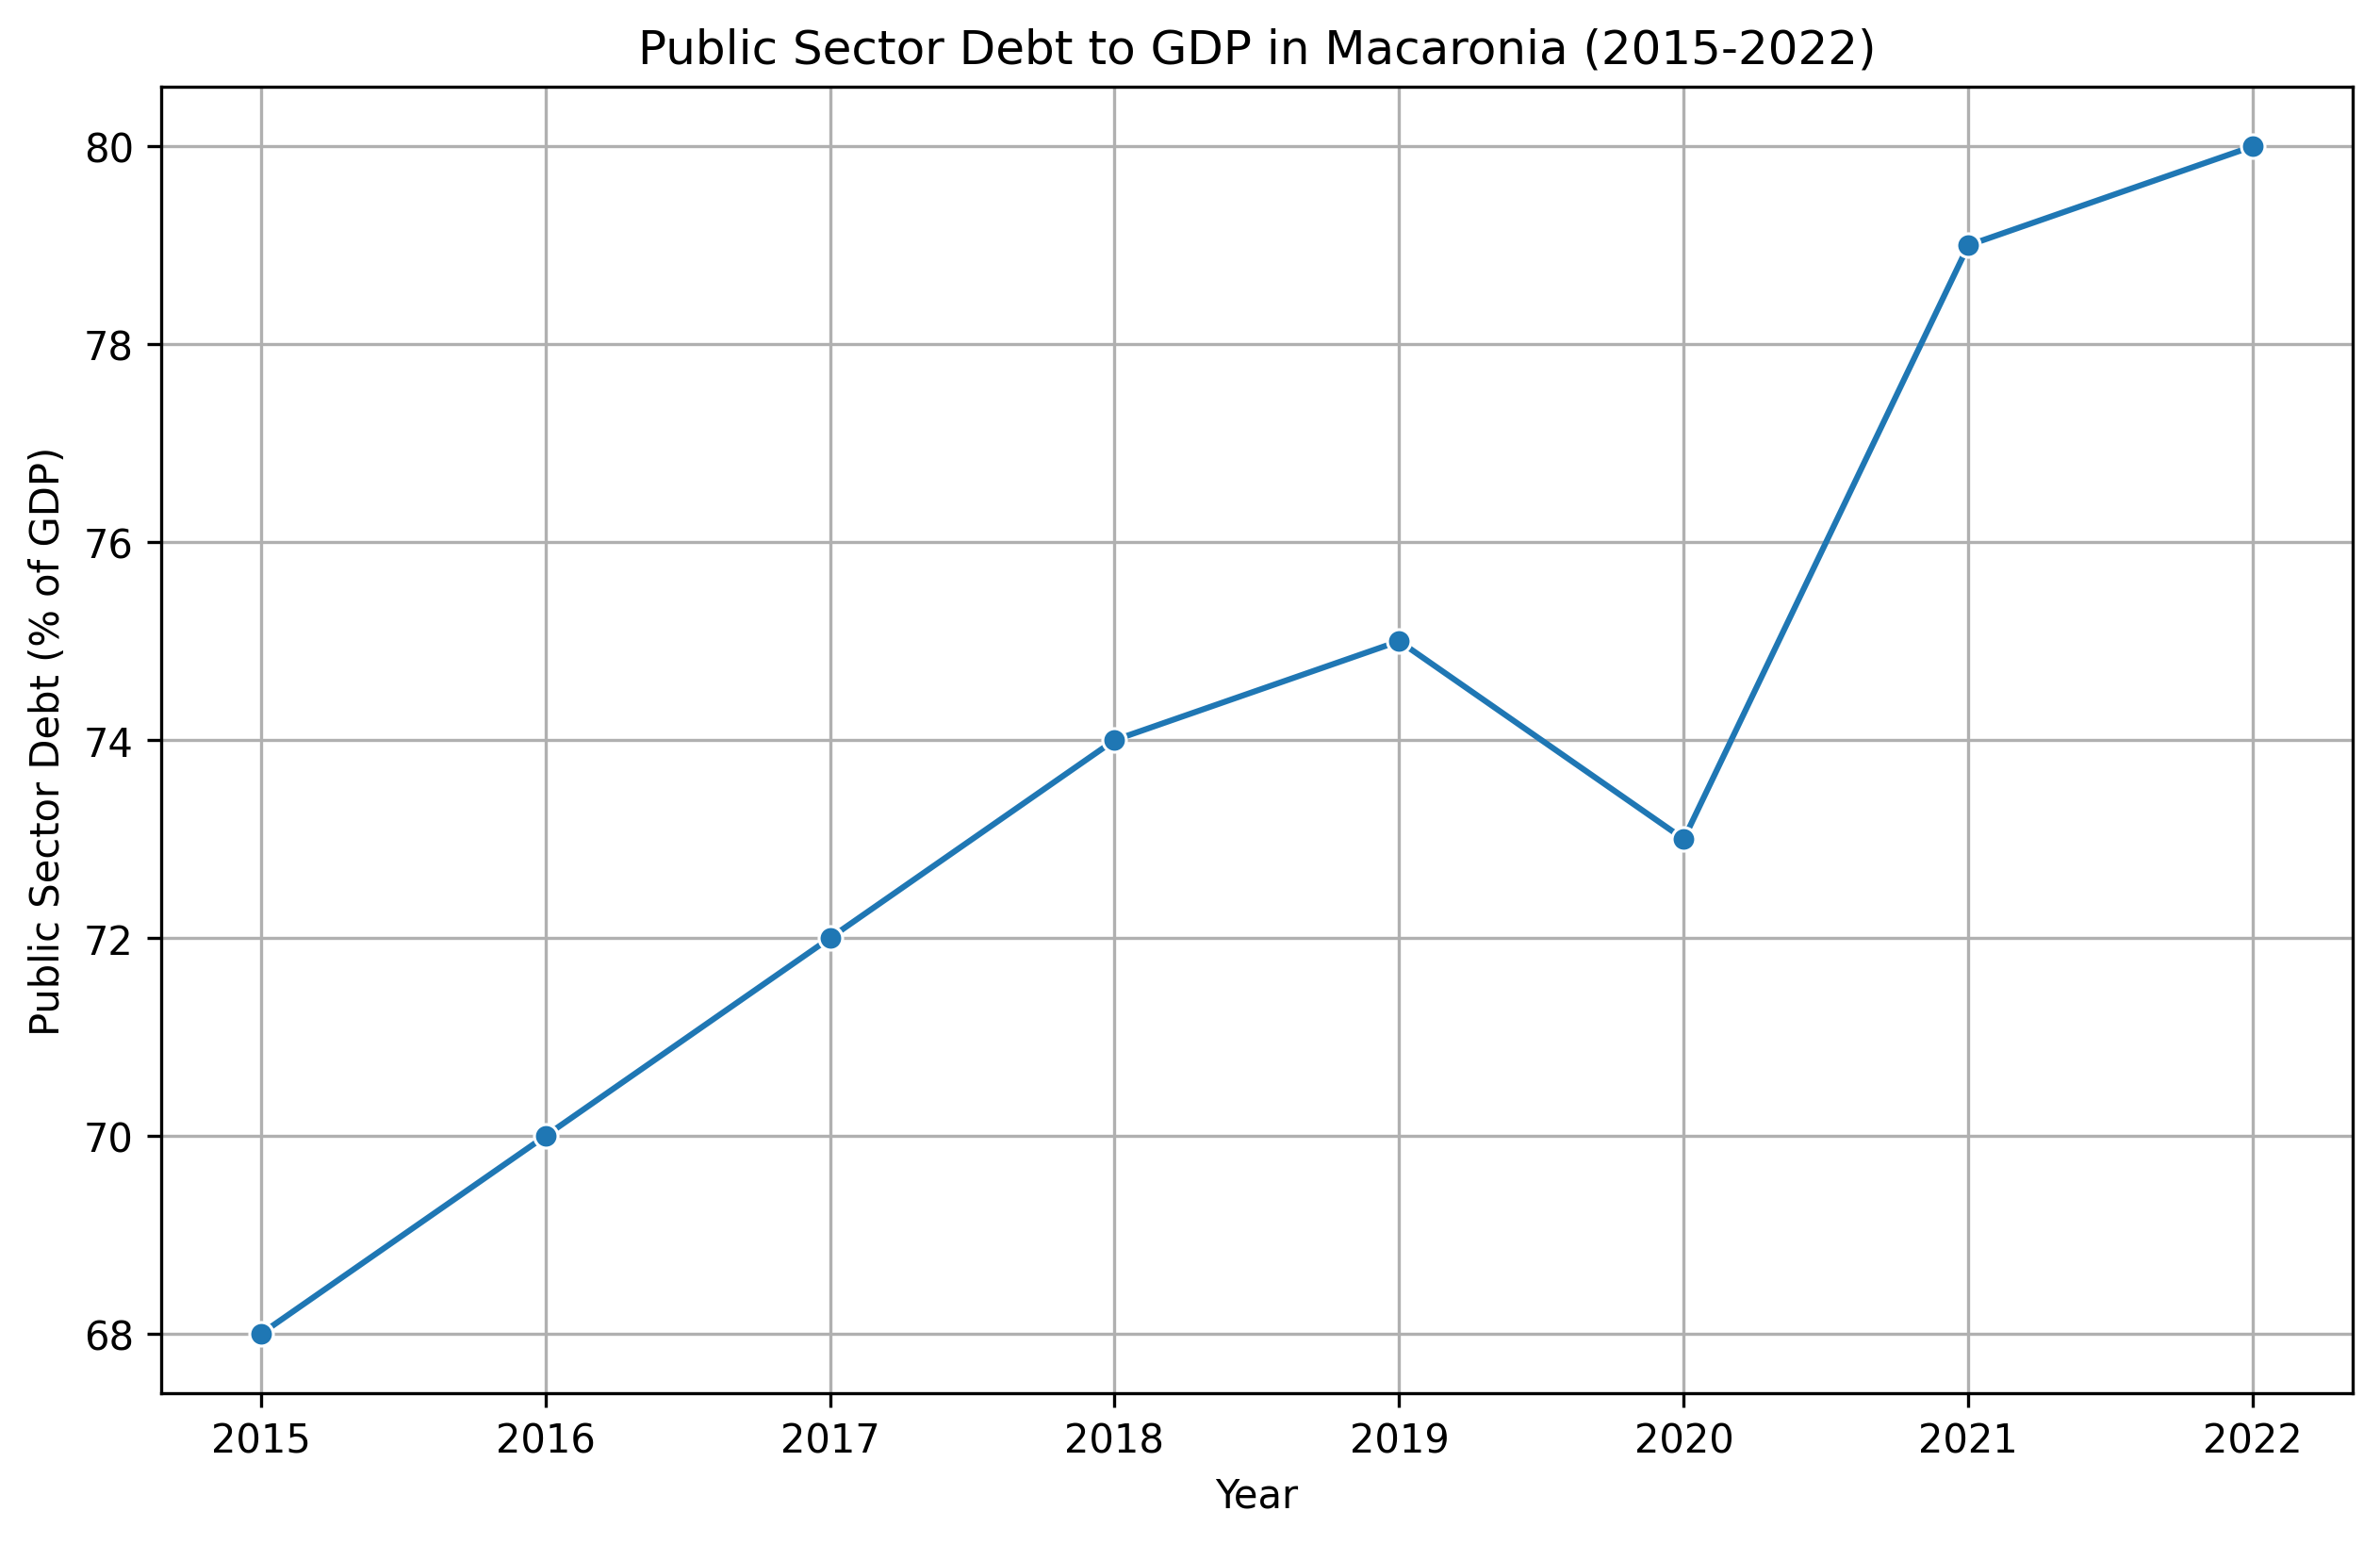
\includegraphics[width=\textwidth]{graph_2.png}
        \caption{\small Public Debt to GDP}
        \label{fig:public_debt_gdp}
    \end{subfigure}
    \caption{Macaronia's REIT Exposure and Public Debt Levels}  % Main figure caption
    \label{fig:reit_debt}
\end{figure}


Given that \textbf{\textcolor{teal}{REITs}} constitute a significant portion of their equity, the risk of \textbf{\textcolor{teal}{insolvency}} is 
substantially higher. A market downturn could trigger a sharp decline in the value of these assets,
eroding the financial institutions' capital bases. To mitigate these risks and strengthen their balance sheets, 
these institutions have resorted to aggressive \textbf{\textcolor{teal}{lending practices}}.

However, the public sector's debt level, which stands at a staggering \textbf{\textcolor{teal}{80\%}} of GDP, 
raises serious concerns about the government's capacity to meet its own financial obligations, 
let alone provide \textbf{\textcolor{teal}{bailouts}} to struggling financial institutions in the event of a crisis. 
In light of this precarious fiscal position, it is essential to move beyond nominal ratios and 
assess the true health of financial institutions by accounting for \textbf{\textcolor{teal}{credit extension}}, 
\textbf{\textcolor{teal}{risk}} and \textbf{\textcolor{teal}{REIT exposure}}.

When these nominal ratios are adjusted, their real value is significantly lower than the nominal figures suggest.
This adjustment uncovers the underlying vulnerabilities in the financial system, emphasizing the urgent need for a more 
accurate assessment of \textbf{\textcolor{teal}{solvency}} and \textbf{\textcolor{teal}{liquidity risks}}.

The adjusted ratio is calculated as:
\begin{equation}
\boxed{
    \text{Adjusted Ratio} = \frac{\text{Nominal Ratio}}{\text{Adjustment Factor}}
}
\end{equation}

To reflect the compounding impact of credit growth, risk exposure and REIT exposure, the adjustment factor is: 

The adjustment factor is calculated as:
\begin{equation}
\boxed{
    \text{Adjustment Factor} = (1 + \text{Credit Growth Rate}) \cdot (1 + \text{Risk Exposure Factor}) \cdot (1 + \text{REIT Exposure})
}
\end{equation}


The risk exposure factor is a subjective measure that reflects the level of risk in the financial system due to factors like economic instblity, 
high levels of debt, or exposure to volatile sectors. In this case, the risk exposure factor is assumed to be 0.5 in 2021 due to the rapid 
credit growth, High REIT exposure and Systemic instability. 



\subsubsection*{Calculations for Banks and Credit Unions real ratios} 



% Increase row height
\renewcommand{\arraystretch}{1.5} % Adjust this value to increase/decrease row height

\begin{table}[h!]
\centering
\begin{tabular}{|>{\centering\arraybackslash}p{4cm}|>{\centering\arraybackslash}p{4cm}|>{\centering\arraybackslash}p{4cm}|} % Centered columns
\hline
\textbf{Parameter} & \textbf{Banks} & \textbf{Credit Unions} \\
\hline
Credit Growth Rate & 0.088 (8.8\%) & 0.132 (13.2\%) \\
\hline
Risk Exposure Factor & 0.5 & 0.5 \\
\hline
REIT Exposure & 0.15 & 0.25 \\
\hline
\textbf{Adjustment Factor} & \textbf{Calculation} & \textbf{Calculation} \\
\hline
& \((1 + 0.088) \times (1 + 0.5) \times (1 + 0.15)\) & \((1 + 0.132) \times (1 + 0.5) \times (1 + 0.25)\) \\
& \(= 1.088 \times 1.5 \times 1.15\) & \(= 1.132 \times 1.5 \times 1.25\) \\
& \(= 1.878\) & \(= 2.122\) \\
\hline
\textbf{Adjusted Real Ratios} & \textbf{Calculation} & \textbf{Calculation} \\
\hline
$\text{Real Liquidity Ratio}_{2021}$ & \(75.0/1.878 = 39.94\) & \(78.8/2.122 = 37.14\) \\
\hline
$\text{Real Adequacy Ratio}_{2021}$ & \(14.8/1.878 = 7.88\) & \(12.8/2.122 = 6.03\) \\
\hline
\end{tabular}
\caption{Adjustment Factor and Adjusted Real Ratios for Banks and Credit Unions (2021)}
\end{table}

The real liquidity ratio for banks stands at \textcolor{teal}{39.94}, and for credit unions, it is \textcolor{teal}{37.14}. Similarly, the real solvency ratio for banks is approximately \textcolor{teal}{7.88}, compared to \textcolor{teal}{6.03} for credit unions. While these ratios may appear stable at first glance, the adjusted figures accounting for \textcolor{teal}{credit growth} and \textcolor{teal}{high-risk asset exposure} reveal a far more concerning reality: both banks and credit unions are \textcolor{teal}{undercapitalized}. This imbalance represents a latent threat within the financial system, one that grows more precarious as external pressures mount.

The parallels to the \textcolor{teal}{2007-2009 financial crisis} are hard to ignore. During that period, undercapitalized institutions were unable to absorb losses when the housing market collapsed, setting off a chain reaction that destabilized the global economy. Today, a similar vulnerability exists. Banks and credit unions, which are meant to serve as pillars of economic stability, could instead become conduits for \textcolor{teal}{systemic risk}. In times of economic stress, their weakened positions could transform them from stabilizers into amplifiers of crisis.

A significant contributor to this risk is the heavy reliance of financial institutions on the \textcolor{teal}{volatile real estate market}. During periods of economic expansion, real estate investments can generate substantial returns, masking underlying weaknesses in balance sheets. However, when market conditions deteriorate, these same investments can quickly become liabilities.

This combination of \textcolor{teal}{undercapitalization} and \textcolor{teal}{overexposure to risky assets} creates the potential for a \textcolor{teal}{domino effect}. If a single institution faces a liquidity or solvency crisis, it could set off a chain reaction, destabilizing the broader financial system. The 2007-2009 crisis demonstrated how the collapse of the housing market could trigger a global recession. In the year 2021 in Macaronia, the same dynamics are at play. Financial institutions, weakened by undercapitalization and over-leveraged portfolios, may struggle to withstand the next economic shock, putting the entire financial ecosystem at risk.

The question is not whether this scenario will unfold, but when. This urgency is further amplified by the fact that Macaronia's economy is \textcolor{teal}{perfectly correlated with global economic growth}, with a correlation coefficient of \textcolor{teal}{1}. This means that any downturn or shock in the global economy will have an immediate and proportional impact on Macaronia, leaving its already fragile financial system even more exposed to \textcolor{teal}{external pressures}.
\textcolor{orange}{\cite{UNCTAD2023FDI}}

\begin{figure}[h]
     \centering
     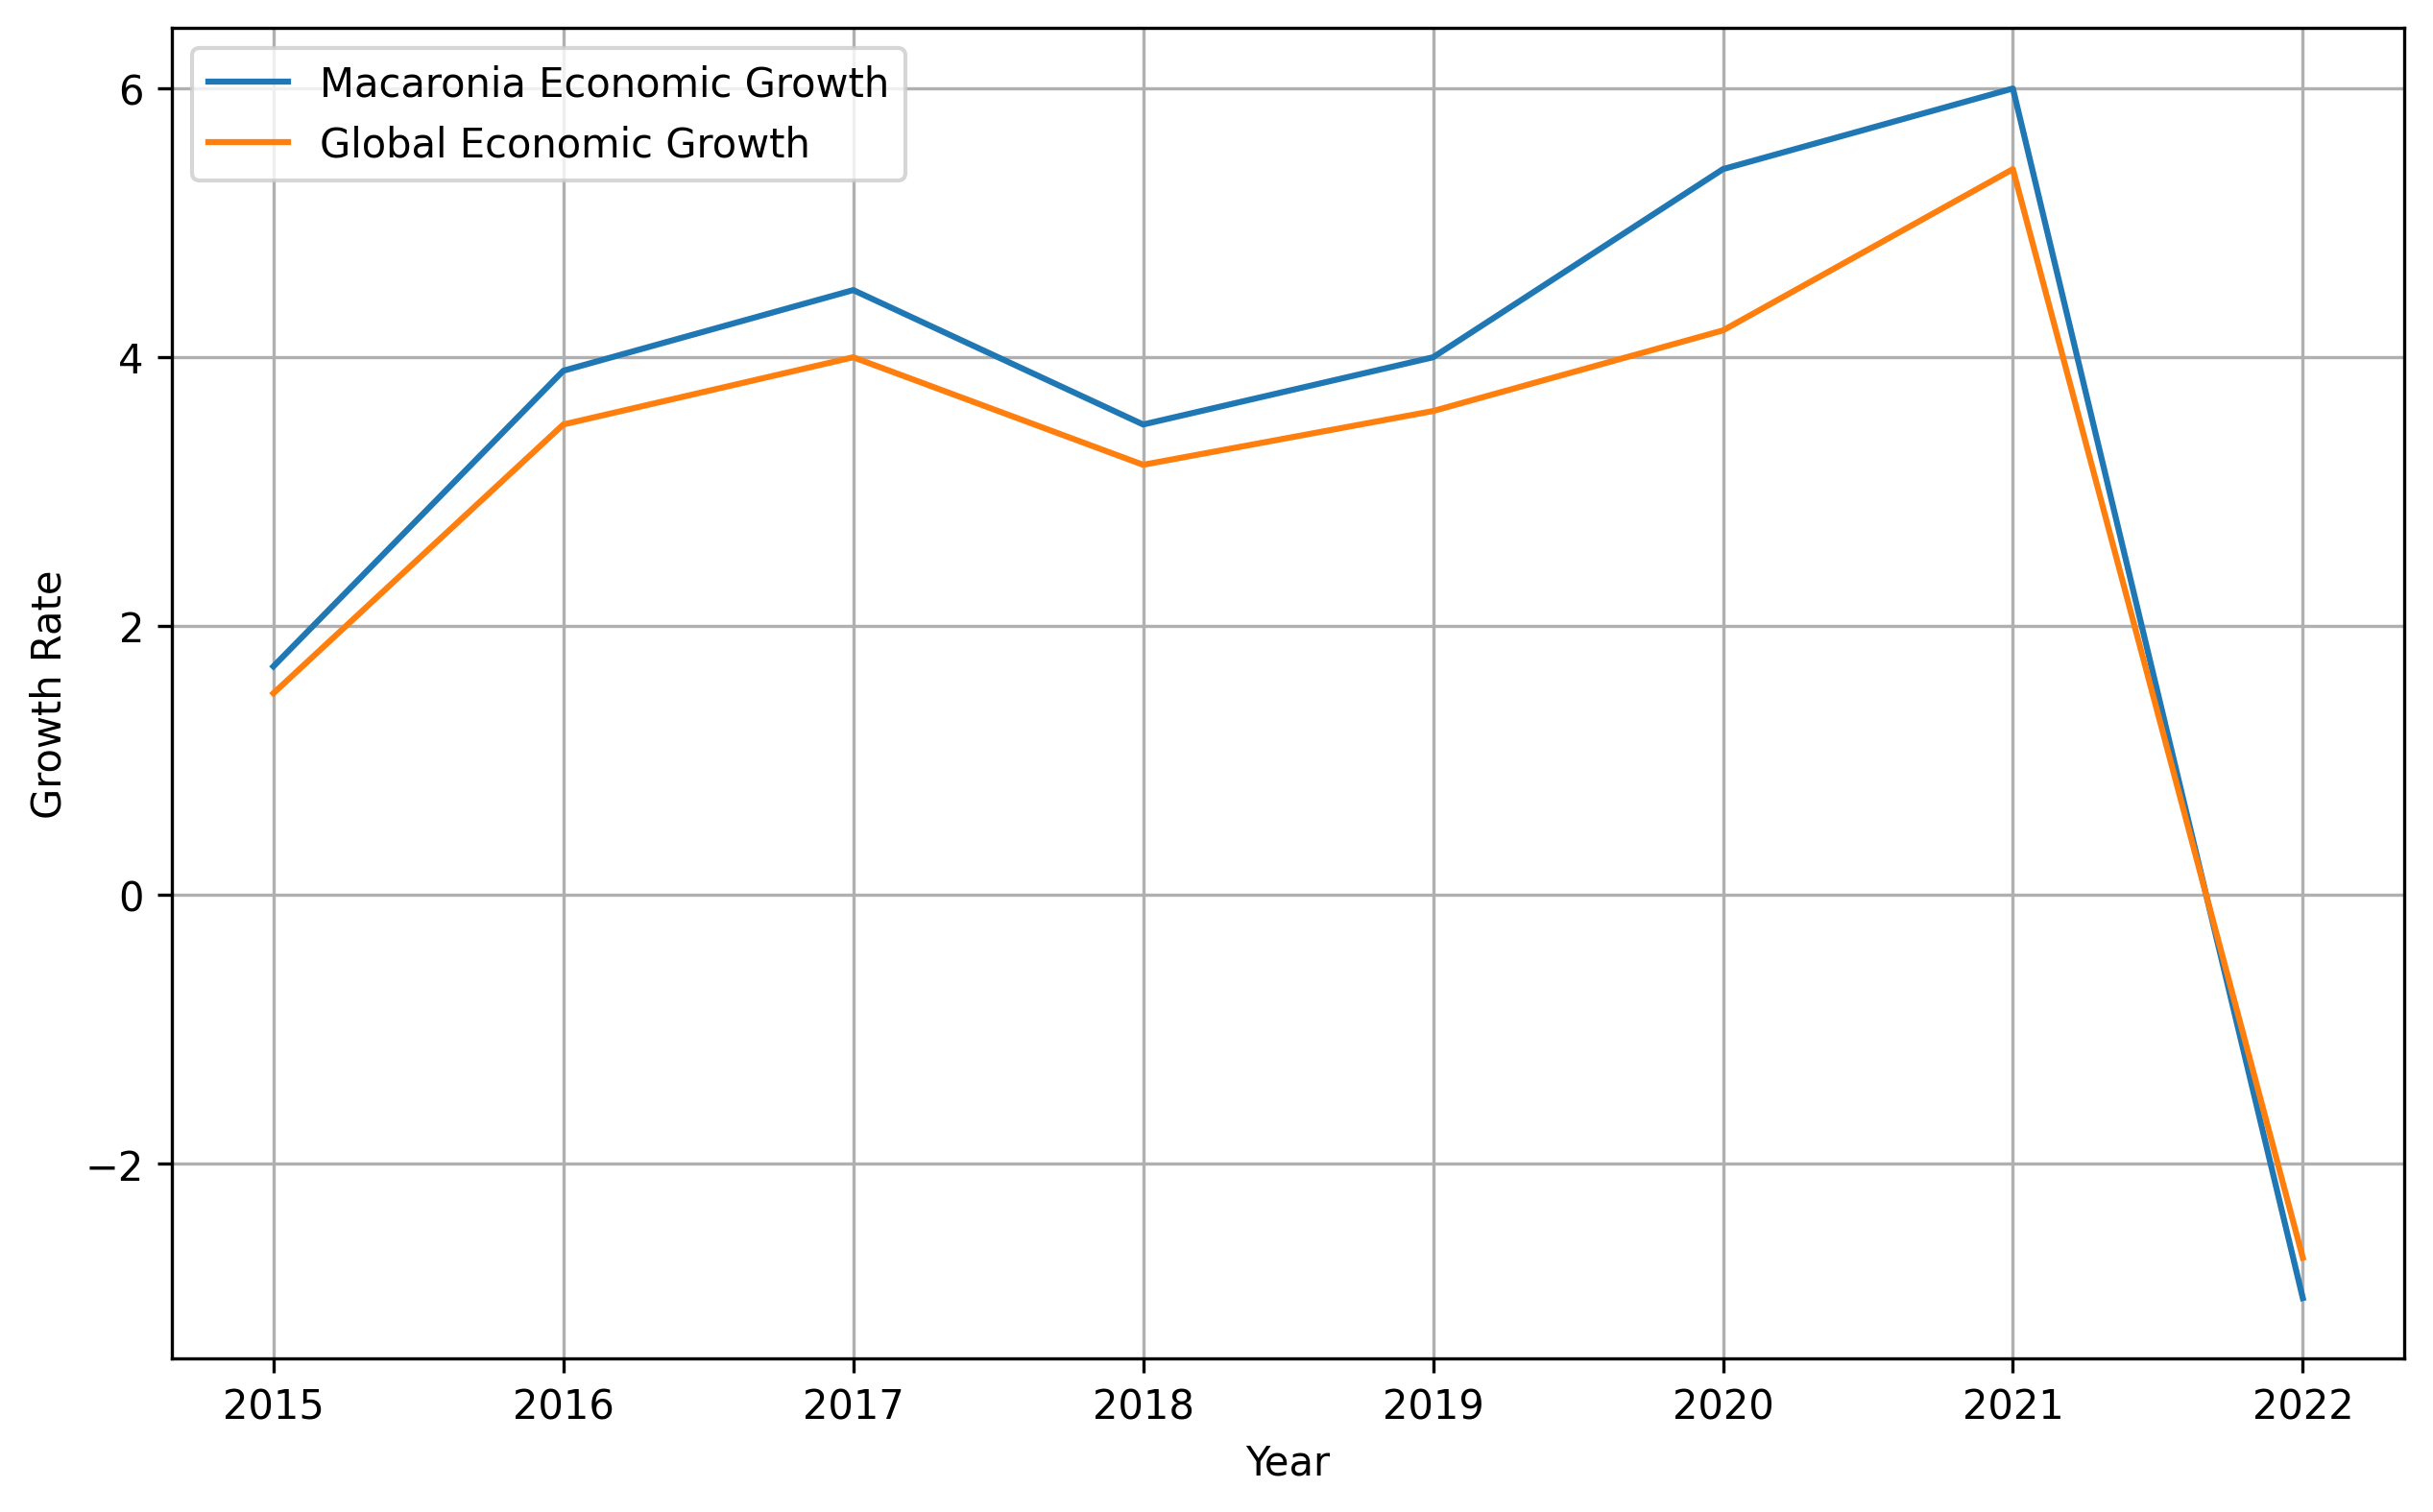
\includegraphics[width=0.5\textwidth]{growth.png}
     \caption{Macaronia Economic Growth vs Global Economic Growth}
     \label{fig:graph_1}
\end{figure}
\subsection*{The Perfect Storm}  

The collapse of a major U.S. financial institution and the ensuing turmoil in global credit markets have brought to light Macaronia's deep-seated vulnerabilities. 
This event sparked widespread uncertainty, prompting international investors to withdraw funds from emerging markets, including Macaronia. The nation’s stock market, cross-listed with U.S. exchanges,
experienced steep declines as capital fled, draining foreign reserves and weakening the national currency. With dwindling reserves, the central bank was unable to supply adequate emergency liquidity,
echoing the struggles seen in countries like \textbf{\textcolor{teal}{Argentina}} and \textbf{\textcolor{teal}{Greece}} during their financial crises.  \textcolor{orange}{\cite{IMF2023WEO}} % CITE: IMF2023WEO

This convergence of external shocks and internal frailties has pushed Macaronia’s financial system to the brink. \textbf{\textcolor{teal}{Undercapitalized banks}}, 
excessive exposure to \textbf{\textcolor{teal}{volatile REITs}}, and a lack of domestic financial resilience have created a fragile ecosystem, highly susceptible to global disruptions. 
The question is no longer if a crisis will occur, but when the next shock will tip the system into chaos. Amid rising global economic uncertainty, the countdown has begun, and the stakes are immense.  



\subsection*{Breakdown of Macaronia's Structural Vulnerabilities}  
Macaronia’s situation reflects a common challenge among Caribbean economies: \textbf{\textcolor{teal}{shallow domestic credit markets}} and limited financial depth.
These structural flaws make such economies highly prone to \textbf{\textcolor{teal}{external shocks}}. As global financial conditions tightened, the nation’s reliance on foreign liquidity 
shifted from a growth engine to a critical weakness. This sudden change laid bare the fragility of its financial system, already strained by undercapitalized banks, heavy investments in volatile REITs, 
and risky lending practices.  \textcolor{orange}{\cite{UNCTAD2023FDI}}



\subsection*{Breakdown of Global Economic Pressures}  
The first signs of trouble appeared as global interest rates rose and \textbf{\textcolor{teal}{credit conditions}} tightened. Higher borrowing costs made it harder for businesses and financial institutions to secure external financing, leading to a sharp drop in \textbf{\textcolor{teal}{foreign direct investment (FDI)}}. The 2007-2009 global financial crisis had already underscored the perils of overreliance on foreign capital. During that period, Macaronia, like other nations dependent on external funding, saw \textbf{\textcolor{teal}{capital flight}} as investors retreated from riskier markets.  

The recent failure of a major U.S. financial institution further destabilized global credit markets, intensifying Macaronia’s challenges. This event triggered a wave of uncertainty, prompting foreign investors to pull out of emerging markets, including Macaronia. The nation’s stock market, tied to U.S. exchanges, plummeted as capital fled, draining foreign reserves and weakening the currency. The central bank, already grappling with shrinking reserves, was unable to provide sufficient emergency liquidity, mirroring the struggles of countries like \textbf{\textcolor{teal}{Argentina}} and \textbf{\textcolor{teal}{Greece}} during their crises.  


\subsection*{Breakdown of Domestic Amplification of External Shocks}  
The global economic downturn, worsened by the U.S. financial institution’s collapse, had immediate and severe domestic consequences. \textbf{\textcolor{teal}{Inflation}}, previously stable, surged to \textbf{\textcolor{teal}{6.0\%}} in 2022, eroding purchasing power and straining household budgets. Simultaneously, \textbf{\textcolor{teal}{unemployment}} rose to \textbf{\textcolor{teal}{8.0\%}}, reflecting the broader economic contraction and fueling social tensions.  

These domestic pressures magnified the impact of external shocks, creating a vicious cycle. Rising inflation and joblessness reduced consumer spending, further weakening the economy. The interplay of global financial disruptions and internal economic distress pushed Macaronia’s financial system to the edge of collapse.  



\subsection*{Breakdown of Financial Sector Vulnerabilities}  
Macaronia’s financial sector, already burdened by heavy exposure to \textbf{\textcolor{teal}{Real Estate Investment Trusts (REITs)}}, faced heightened challenges as global credit markets tightened. Falling REIT values caused significant losses for banks and credit unions, many of which had heavily invested in these volatile assets. This triggered a \textbf{\textcolor{teal}{liquidity crunch}}, as institutions struggled to maintain adequate reserves and meet short-term obligations.  

The U.S. financial institution’s collapse served as a stark reminder of how declining asset values, particularly in real estate, can ignite widespread financial instability. In Macaronia, the effects were immediate: the stock market plunged, capital flight accelerated, and the currency came under intense pressure. With limited reserves, the central bank was unable to stabilize the situation, leaving the financial system dangerously exposed.  



\subsection*{Breakdown of Structural Weaknesses}  
Macaronia’s financial system was further crippled by deep-rooted structural flaws. High \textbf{\textcolor{teal}{collateral requirements}} and limited access to domestic credit, particularly for small and medium-sized enterprises, stifled economic growth and reinforced reliance on external financing. As global credit conditions tightened, this dependence became a critical liability.  

The absence of robust \textbf{\textcolor{teal}{macroprudential oversight}} also played a key role in the crisis. Unlike nations with strong systemic risk monitoring frameworks, such as those 
under the \textbf{\textcolor{teal}{European Systemic Risk Board}}, Macaronia lacked effective mechanisms to identify and address vulnerabilities. This left the country unprepared to manage the cascading failures 
triggered by global financial disruptions.  \textcolor{orange}{\cite{ECB2023ESRB}}


